%!TEX root = main.tex

\chapter{Desarrollo de la solución}

\section{Velocidad del viento}
\subsection{Modelo Matemático} \label{ss:Modelo_Mat}
Como se adelanta anteriormente, para encontrar los parámetros de la distribución de Weibull que se ajusten a los datos de prueba se utilizará el \emph{Particle Swarm Optimization}. La función de distribución de Weibull está definida en la ecuación \ref{eq:weibull}. El PSO a utilizar está representado por la ecuación \ref{eq:PSO}. La función objetivo se describe con la fórmula \ref{eq:PSO_FO} y es aquella con la que se busca minimizar el error cuadrático entre la frecuencia real de los datos y la estimada por la distribución de Weibull. Los parámetros a encontrar $k$ y $c$ deben ser $\geq 0$ . Por último, a modo de favorecer la exploración al comienzo y la explotación al final de las iteraciones del PSO, se utilizará la recomendación de \cite{Carneiro15} para la variación de parámetros del enjambre:
\begin{align}\label{eq:VariationParameters}
    w(j) &= (1 - \frac{j}{iter_{max}})^{\alpha}(w_{max} - w_{min} + w_{min})\\
    c_{1}(j) &= (1 - \frac{j}{iter_{max}})^{\beta}(c_{1max} - c_{1min}) + c_{1min}\\
    c_{2}(j) &= (1 - \frac{j}{iter_{max}})^{\gamma}(c_{2min} - c_{2max}) + c_{2max}
\end{align}    
Donde $w_{max} = 0.9$ y $w_{min} = 0.4$, $c_{1max}$, $c_{2max}$ y $c_{1min}$, $c_{2min}$ son 2.5 y 0 respectivamente. Los parámetros $\alpha, \beta, \gamma$ son definidos como 0.5, 1.5 y 1.0 respectivamente. $iter_{max}$ es el máximo número de iteraciones.

\subsection{Representación}
Cada vector posición de las partículas del enjambre representa una solución candidata la cual varía dentro de cierto espacio de búsqueda definido por los límites de las componentes. Así, para el caso de los parámetros de la distribución de Weibull, la posición de las partículas está representada por los parámetros $k$ y $c$ quedando de la forma:
\begin{align}
    x = (k, c)
\end{align}    
Para ambos parámetros, se establecen los límites entre $0 \leq (k,c) \leq 20$, criterio que se basa en el trabajo de Carneiro et al. \cite{Carneiro15}. De esta forma, las partículas se moverán dentro de ese rango, manteniéndose en los lugares que minimizan la función objetivo, la cual representa el error de la predicción de Weibull versus los datos reales.\\
Así, para cada partícula se define una estructura que posee las siguientes propiedades: 
\begin{enumerate}\label{rep:Particle}
    \item Posición: vector de números flotantes de largo dos, los cuales representan la ubicación de la partícula dentro del espacio de búsqueda y sus componentes a los parámetros $k$ y $c$.
    \item Velocidad: vector de números flotantes que representan el cambio de valor de cada componente de la posición de la partícula en determinada iteración. Se actualiza en base a la ecuación de velocidad del PSO.
    \item Mejor resultado personal: vector flotante que guarda la mejor posición conseguida por la partícula durante las iteraciones transcurridas.    
\end{enumerate}        
Mientras que el enjambre, siendo esencialmente una estructura que posee referencia a todas las partículas, queda representado de la siguiente forma:
\begin{enumerate}\label{rep:Swarm}
    \item Partículas: Arreglo de referencias a las estructuras de partículas creadas.
    \item Mejor posición global: De todos los mejores resultados particulares a cada partícula, se almacena la mejor posición de todas. La que persiste al final del ciclo de iteraciones, es la solución final.
    \item W, C1 y C2: Son los parámetros de inercia, cognitivo y social respectivamente.    
\end{enumerate} 

\subsection{Descripción del algoritmo}
La lógica del algoritmo \ref{alg:pso} se basa en mover las partículas dentro del rango definido para los componentes de la solución hasta que todas las partículas se concentren en alguna zona que represente una buena solución al problema, no necesariamente el óptimo. Lo importante en cada iteración es actualizar o mover el enjambre, revisar y guardar las mejores soluciones y actualizar los parámetros de inercia, cognitivo y social que definen las velocidades.
%!TEX root = main.tex

\begin{algorithm}[h!]
\caption{PSO para el ajuste de los parámetros de la distribución de Weibull}
\label{alg:pso}
\begin{algorithmic}
\REQUIRE Datos de frecuencias de velocidades del viento.
\ENSURE Valores para los parámetros $k$ y $c$.
\STATE enjambre = inicializar(w,c1,c2)
\FOR{$i = 1$ to $Iter_{max}$}
\FOR{Each partículas en enjambre}
    \STATE actualizarVelocidadPartícula(partícula)
    \STATE actualizarPosiciónPartícula(partítucla)
    \STATE guardarMejorResultadoPartícula(partícula)
\ENDFOR
\STATE guardarMejorResultadoGlobal(enjambre)
\STATE actualizarParámetros(enjambre)
\ENDFOR
\STATE retornarMejorResultadoGlobal(enjambre).
\end{algorithmic}
\end{algorithm}

Las iteraciones fueron probadas hasta un máximo de 1000 y 50 partículas, (A excepción del experimento donde se consideraron todos los promedios diarios, 2013, 2014 y 2015, en el cual, se utilizaron 200 partículas). Los parámetros de $w$, $c1$ y $c2$ fueron definidos tal y como explica en el modelo matemático, en la sección \ref{ss:Modelo_Mat}.\\

\subsection{Experimentos}\label{sec:Experimentos_velocidad}
Los experimentos fueron realizados con datos del viento obtenidos por la Armada de Chile para la región de Valparaíso en los años 2013, 2014 y 2015. Estos fueron tratados mediante \emph{scripts} desarrollados en python para obtener las frecuencias de las distintas velocidades del viento registradas a lo largo del año. Los datos se organizaban de la siguiente forma: Por cada año, se tiene una tabla en un archivo exel de cada mes, en donde se registra por cada fila los resultados de la medición de cada día. Las mediciones son registradas en un intervalo de tres horas, es decir, se tienen registros diarios para las 3:00, 6:00, 9:00, 12:00, 15:00, 18:00, 21:00 y 00:00 horas.\\
Un ejemplo es la tabla mostrada en la figura \ref{fig:example_data}.
 \begin{figure}[h!]
    \centering
    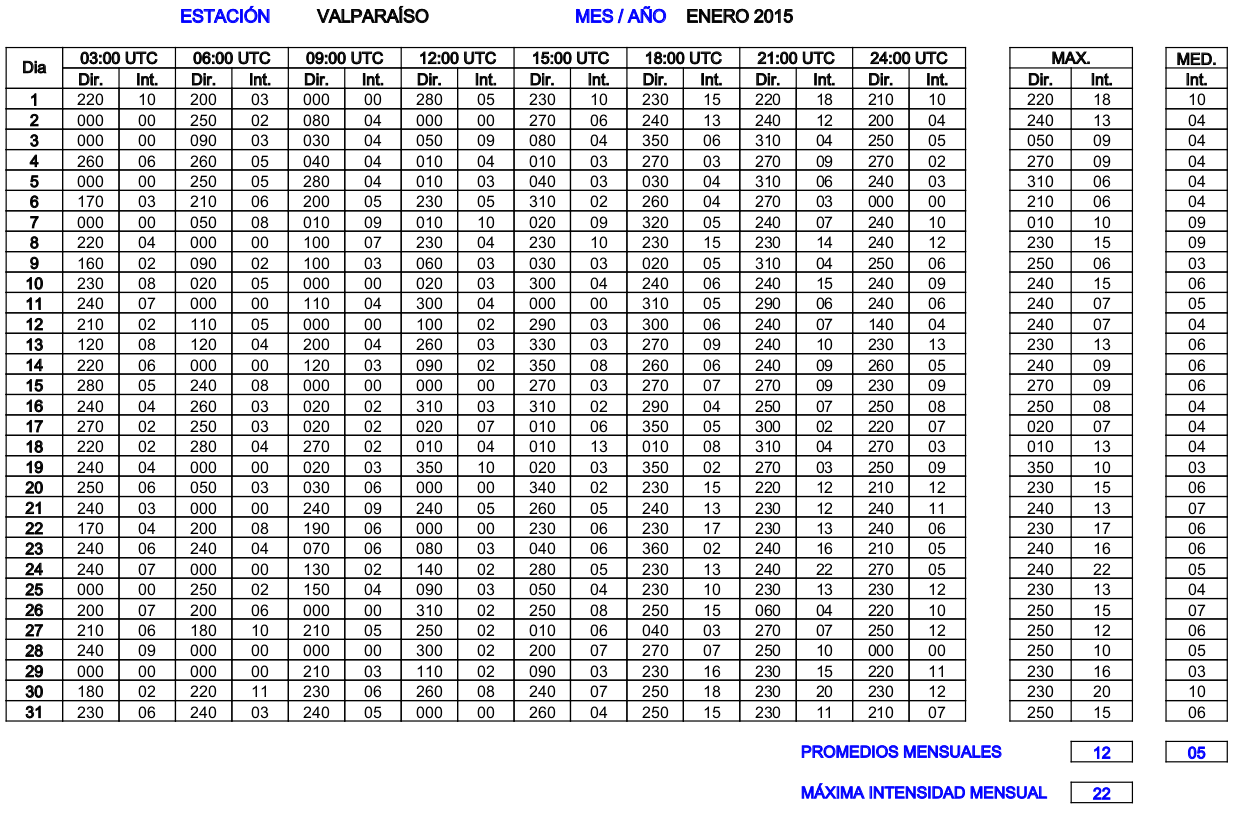
\includegraphics[height=100mm]{figures/example_data.png}
    \caption{Ejemplo colección de datos Enero Valparaíso 2015}
    \vspace{-.25cm}
    \caption*{Obtenido desde el Instituto Meteorológico de la Armada de Chile.}
    \label{fig:example_data}
 \end{figure}
El ajuste de la distribución de Weibull a estos datos de velocidad del viento se hizo considerando las siguientes configuraciones para el cálculo del
histograma de frecuencias:
\begin{enumerate}
	\item \textbf{Todos los años}. Se considera el promedio diario de velocidad del viento como dato unitario para el cálculo de las frecuencias, considerando
	todos los días en el intervalo de Enero del 2013 hasta Diciembre del 2015.
	\item \textbf{Anual}. Se considera el promedio diario de velocidad del viento como dato unitario para el cálculo de las frecuencias en
	un lapso anual (2013, 2014 y 2015).
	\item \textbf{Por temporada}. Se considera el promedio diario de velocidad del viento como dato unitario para el cálculo de las frecuencias en
	un lapso de tres meses (Enero - Marzo ; Abril - Junio; Julio - Septiembre; Octubre - Diciembre).
	\item \textbf{Datos brutos}. Se considera cada medición realizada (8 por día) como dato unitario, en un lapso de un año.
\end{enumerate}

Una vez obtenido los datos de frecuencias, se procede a aplicar el algoritmo PSO obteniendo los parámetros de ajuste $k$ y $c$. De esta manera, se evalúa la calidad del modelo generado (distribución de Weibull), para las distintas configuraciones mediante gráficos y los siguientes test estadísticos (utilizados en el trabajo de Carneiro et al. \cite{Carneiro15}):
\begin{enumerate}
    \item \emph{Root Mean Square Error}
        \begin{align}
            RMSE = \sqrt{\frac{\sum_{i=1}^{N}(X_i - Y_i)^2}{N}}
        \end{align}    
    \item \emph{Correlation}
        \begin{align}
            r = \frac{\sum_{i=1}^{N}(X_i - X_{med})\cdot(Y_i - Y_{med})}{\sqrt{\sum_{i=1}^{N}(X_i - X_{med})^2}\cdot\sqrt{\sum_{i=1}^{N}(Y_i - Y_{med})^2}}
        \end{align}    
    \item \emph{Relative Bias}
        \begin{align}
            RB = \frac{X_{med} - Y_{med}}{Y_{med}}  
        \end{align}    
\end{enumerate}        
Donde $N$ es el número de datos, $Y_i$ la frecuencia de dichos datos, $X_i$ la frecuencia entregada por la distribución de Weibull, $X_{med}$ la media de $X_i$ e $Y_{med}$ la media de $Y_i$. \\

Las pruebas fueron realizadas en un computador con sistema operativo Ubuntu 16.04 64-bit, 3.8 GB de memoria y procesador doble núcleo Intel Pentium 2.60 GHz. 

\section{Dirección del viento}
\subsection{Modelo Matemático} 
Como se comenta anteriormente, la distribución de densidad de probabilidad que se utilizará para describir la distribución de datos de dirección del viento
es la \emph{mixture von mises distribution} descrita en \ref{eq:mixtureVonMises}, la cual consiste básicamente en una combinación lineal de la \emph{simple von Mises distribution} descrita en \ref{eq:simpleVonMises}.\\ 
De forma preliminar, los datos se ordenan en un histograma de densidad con el cual se obtiene un esqueleto de la distribución de densidad de probabilidad. Posteriormente se requieren encontrar los parámetros de ajuste $\mu_j$, $k_j$ y $w_j$ para cada $j$-ésima \emph{simple von Mises distribution}. La forma en que
se realiza esto último en este trabajo está basado en José A. Carta et al. \cite{Carta07} y se describe a continuación.\\
Para la construcción del histograma se divide el rango de datos que va de 0 a $2\pi$ en $T$ clases con frecuencia $O_i$ la cual representa la suma de las observaciones en el rango de la clase $T$. Posteriormente se definen $k$ sectores del mismo largo desde las $T$ clases, relacionados al número de direcciones de viento predominantes (o con mayor frecuencia). Esto define el número de funciones de von Mises a utilizar. La estimación de $k$ se realiza mediante la observación del histograma generado, un análisis cualitativo de las direcciones predominantes en los datos.\\
Para la aproximación inicial de los parámetros de la \emph{mixture von mises distribution} se utiliza una estimación numérica basada en los datos recolectados acerca de la dirección del viento.\\
Sea $j \in \{1 ... k\}$ el subíndice del sector representado por la $j$-ésima función de von Mises.\\
La dirección del viento predominante $\mu_j$ se estima de la siguiente forma:
\begin{align}\label{eq:Prevailing_Param}
    \mu_j &= 
        \left\{
            \begin{array}{ll}
                arctan(\frac{s_j}{c_j})  & s_j \geq 0, c_j > 0\\
                \frac{\pi}{2} & s_j > 0, c_j = 0\\
                \pi + arctan(\frac{s_j}{c_j}) & c_j < 0\\
                \pi & s_j > 0, c_j = -1\\
                2\pi + arctan(\frac{s_j}{c_j}) & s_j < 0, c_j > 0\\
                3\frac{\pi}{2} & s_j < 0, c_j = 0\\
            \end{array}
        \right.
\end{align}
En donde $s_j$ y $c_j$ representan el seno y coseno promedio del sector $j$.\\
Tradicionalmente, se estima el parámetro de concentración $k_j$ con la ecuación:
\begin{align}\label{eq:Implicit_Param}
    \frac{I_1(k_j)}{I_0(k_j)} = \sqrt{s_j^2 + c_j^2}
\end{align}
Donde $I_1(k_j)$ es la función modificada de Bessel de primera clase y orden 1.
 Como se explica en Banerjee et al. \cite{Banerjee05}, debido a la falta de una solución análitica a la ecuación \ref{eq:Implicit_Param}, no es posible estimar directamente los valores de $k$. Se podrían utilizar métodos para ecuaciones no lineales, pero para datos de altas dimensiones, problemas de desbordamiento (\emph{overflow}) o inestabilidad numérica se vuelven concurrentes. Por tanto, se utiliza la propuesta realizada en el trabajo de Heckenbergerova et al. \cite{Heckenbergerova15} con lo cual el parámetro $k_j$ puede ser aproximado por:\\
\begin{align}
    |k_j| = \{23.29041409 - 16.8617370\sqrt[4]{s_j^2 + c_j^2}\} 
\end{align}
Los pesos iniciales $w_j$ son aproximados como: \\
\begin{align}\label{eq:Weight_Param}
    w_j = \frac{\sum_{i=J_l}^{J_u} O_i}{\sum_{i=1}^{T} O_i}
\end{align}

Donde $J_l$ y $J_u$ son los índices de los bordes del sector $j$.\\
Esta estimación inicial de los parámetros de la \emph{mixture von mises distribution} es mejorada mediante la meta-heurística \emph{Particle Swarm Optimization}. Para el PSO se utiliza la representación descrita en \ref{eq:PSO} y la modificación a este sugerida en Carneiro et al. \cite{Carneiro15} descrita previamente en \ref{eq:VariationParameters}.\\
La función objetivo para el PSO es el test estadístico $\chi^2$ descrito en \cite{Heckenbergerova15} como sigue a continuación:
\begin{align}\label{eq:FO_Direction}
    \chi^2 = \sum_{i=1}^{T}\frac{(O_i - np_{i})^2}{np_i}
\end{align}
Donde $T$ es el número de clases de frecuencia definido para construir el histograma, $n$ es la suma de las frecuencias observadas $O_i$ y $p_i$ es la probabilidad teórica de cada clase de frecuencia predicha por el modelo ajustado.\\
Para el cálculo del $p_i$ se utiliza:
\begin{align}
    p_i = \int_{l_i}^{u_i} f(x) dx
\end{align}
Donde $u_i$ y $l_i$ son los bordes de la $i$-ésima clase de frecuencia.\\
La forma de la solución a encontrar es descrita en \ref{eq:sol_pso}. Esta es restringida por la condición para los pesos de la \emph{mixture von mises distribution}, la cual obliga a que se deba cumplir que la suma de los pesos sea igual a 1, como se describe en \ref{eq:WeightConstraint}.
\subsection{Representación}\label{sec:Representacion}
La representación del PSO es similar al utilizado para el ajuste de la distribución de datos de velocidad del viento. Las partículas y el enjambre están representados por \ref{rep:Particle} y \ref{rep:Swarm} respectivamente.\\
La solución para el PSO que mejora la estimación inicial de los parámetros para la \emph{mixture von Mises distribution} está representado por un vector $v$ en el cual se encuentran los valores para todos los parámetros de cada \emph{simple von Mises distribution}. Estos valores están codificados para que el algoritmo se mueve en el rango desde 0 a 1.\\
El vector solución tiene la forma:
\begin{align}
    v = (\overbrace{v_1,...,v_k}^{\mu},\overbrace{v_{k+1},...,v_{2k}}^{k},\overbrace{v_{2k+1},...,v_{n}}^{w}).
\end{align}
El parámetro $\mu$ está representado en el rango $i \in \{1,...,k\}$ y para ser decodificado debe ser escalado por $2\pi$.\\
El parámetro $k$ está representado en el rango $i \in \{k+1,...,2k\}$ y para ser decodificado debe ser escalado por $[0, 700]]$.\\
El parámetro $w_j$ está representado en el rango $i \in \{2k+1,...,n\}$ cuyos valores van en el rango $[0,1]$.

\subsection{Descripción del algoritmo}
El algoritmo para el ajuste de la función de densidad de probabilidad para la dirección del viento se basa en la propuesta de Heckenbergerova et al. \cite{Heckenbergerova15}.\\ 
Como se ha ido vislumbrado, consiste en dos fases. La primera, una aproximación basada en la estimación numérica de los parámetros requeridos para la \emph{mixture of von Mises distribution} a través de operaciones simples con los datos recolectados, y la segunda, una mejora de la solución inicial obtenida en la fase anterior mediante el uso de la meta-heurística \emph{Particle Swarm Optimization}. \\
El algoritmo para la aproximación inicial de la solución se describe en \ref{alg:init_aprox_direction}.
%!TEX root = main.tex

\caption{Aproximación inicial de los parámetros de la \emph{mixture von Mises distribution}}
\begin{algorithmic}
\REQUIRE Datos de frecuencias de la dirección del viento.
\REQUIRE K, Cantidad de \emph{simple von Mises distribution}.
\REQUIRE T, clases de frecuencias.
\REQUIRE D, Total de datos.
\ENSURE Valores para los parámetros $\mu_j$, $k_j$ y $w_j$, para cada $j \in \{1,...,k\}$.
\STATE sol = inicializarVectorSolución(3*K)
\FOR{$j = 0$ to $K$}

\STATE datos$_j$ = datosEnRango($j*D/K$)
\STATE s$_j$ = obtenerSenoPromedio(datos$_j$)
\STATE c$_j$ = obtenerCosenoPromedio(datos$_j$)
\STATE u$_j$ = obtenerDirecciónPredominante(s$_j$,c$_j$)
\STATE k$_j$ = obtenerConcentración(s$_j$, c$_j$)
\STATE w$_j$ = obtenerPeso($j*(T/K)$, $(j + 1)*(T/K)$)
\STATE addToSolution(sol, u$_j$, k$_j$, w$_j$)

\ENDFOR
\STATE retornarSoluciónInicial(sol).
\end{algorithmic}
En donde la estimación de los parámetros se realiza como se describe en \ref{eq:Prevailing_Param} para los $\mu_j$, \ref{eq:Implicit_Param} para los $k_j$ y \ref{eq:Weight_Param} para los pesos $w_j$.
Una vez obtenida la aproximación inicial se procede a mejorar esta mediante el uso del PSO.
%!TEX root = main.tex
\caption{PSO para la mejora de la aproximación de los parámetros de la \emph{mixture von Mises distribution}}
\begin{algorithmic}
\REQUIRE Datos de la dirección del viento.
\REQUIRE Solución inicial para el ajuste de la \emph{mixture von Mises distribution}.
\ENSURE Solución inicial mejorada.
\STATE enjambre = inicializar(w,c1,c2)
\FOR{$i = 1$ to $Iter_{max}$}
\FOR{Each partículas en enjambre}
    \STATE actualizarVelocidadPartícula(partícula)
    \STATE actualizarPosiciónPartícula(partítcula)
    \STATE revisarLímitesPosición(partícula)
    \STATE guardarMejorResultadoPartícula(partícula)
\ENDFOR
\STATE guardarMejorResultadoGlobal(enjambre)
\STATE actualizarParámetros(enjambre)
\ENDFOR
\STATE retornarMejorResultadoGlobal(enjambre).
\end{algorithmic}
El algoritmo es bastante similar en estructura al desarrollado para la velocidad del viento \ref{alg:pso}. Sin embargo,
existen diferencias importantes, relevantes al problema actual que se destacarán a continuación.\\
Para la inicialización de las partículas, se realizaron pequeñas perturbaciones a la solución inicial tal y como se sugiere en Heckenbergerova et al. \cite{Heckenbergerova15}. Esto evita que la solución escape a zonas que tengan un buen resultado en la función objetivo, pero que la forma escape a la del histograma. Debido a que la función objetivo definida \ref{eq:FO_Direction} mide las diferencias de frecuencias entre los datos reales y los teóricos, es decir, las áreas de las barras del histograma de densidad versus el área bajo la curva de la distribución de probabilidad en algún intervalo, más de una forma de la curva podría parecer una buena solución. (referencia imagen) Por ello, la idea es mantener la forma inicial encontrada, mejorándola sin deformarla. Así, las perturbaciones iniciales a los valores entre 0 y 1  de las posiciones de las partículas eran del orden de $~ 10^{-3}$.\\
La forma en que se cuidaron las condiciones de borde consistieron en limitar el avance de las partículas a los bordes 0 y 1 manteniéndolos en dichos valores si es que se excedían a ellos.\\
Para cuidar la restricción de pesos se normalizaran los valores determinados en cada iteración, es decir, se suman todos los valores $w_j$ y se ponderan dichos valores por el recíproco de la suma obtenida.\\
Debido a que la función objetivo implica determinar la frecuencia teórica, es necesario determinar la probabilidad
de cierto rango de direcciones mediante el cálculo del área bajo la curva de la distribución de densidad de probabilidad para luego ser multiplicada por la suma del total de datos y así obtener el valor requerido. Por ende, para el cálculo de la integral se utilizaron sumas de Riemann con una partición conveniente al desempeño del algoritmo y la precisión requerida.\\
Finalmente, la solución obtenida es decodificada tal y como se explica en la sección anterior \ref{sec:Representacion}.\\
%%Ver redacción acá ....

\subsection{Experimentos}
Similar a los descrito en \label{sec:Experimentos_velocidad}, los datos de dirección del viento son tratados para rescatar las mediciones pertinentes al trabajo aquí expuesto. Estos se encuentran inicialmente en un formato como el que se puede apreciar en la figura \ref{fig:example_data}.\\
Nuevamente, las pruebas fueron realizadas en un computador con sistema operativo Ubuntu 16.04 64-bit, 3.8 GB de memoria y procesador doble núcleo Intel Pentium 2.60 GHz.\\
Para evaluar la calidad de la solución, se utiliza el test \emp{Chi square goodness fit}\cite{goodFitTest}, con lo cual se evalúa que tan bien representa el modelo propuesto a los datos medidos. Para ello, la hipótesis nula $H_0$ es que los datos de dirección del viento se distribuyen según la función \emph{mixture of von Mises distribution} y la hipótesis alternativa $H_1$ niega dicha afirmación. Se rechaza $H_0$ si el valor de la función objetivo del PSO para la solución final encontrada excede el valor crítico de $\Xi^2$ para un nivel de significancia de $\alpha = 0.05$ y 13 grados de libertad, es decir \textbf{22.362}, el cual se puede encontrar en la tabla de la distribución $\Xi^2$ \cite{chiSquareTable}. Los grados de libertad son definidos a partir de la cantidad de clases de frecuencia definidas para el estudio, en este caso, se dividió el rango de valores de $\[0, 2\pi\]$ en 14 tramos iguales, por lo quedan $(n-1)$ grados de libertad, 13 en este caso.\\
Los experimentos realizados...

%%Mayor numero de clases disminuye la precisión y hace el algoritmo más lento.... 
\section{Aplicación de los algoritmos propuestos}
El esquema \ref{esq:PSO_DIR} resume el funcionamiento del algoritmo.
%% Los parámetros....
\begin{figure}[ht!]
\caption{Esquema de uso del algoritmo}
% Define block styles
\tikzstyle{decision} = [diamond, draw, fill=blue!20, 
    text width=4.5em, text badly centered, node distance=3cm, inner sep=0pt]
\tikzstyle{block} = [rectangle, draw, fill=blue!20, 
    text width=15em, text centered, rounded corners, minimum height=4em]
\tikzstyle{blockALG} = [rectangle, draw, fill=green!20, 
    text width=15em, text centered, rounded corners, minimum height=4em]
\tikzstyle{line} = [draw, -latex']
\tikzstyle{cloud} = [draw, ellipse,fill=red!20, node distance=7cm,
    minimum height=2em]
    
\begin{tikzpicture}[node distance = 3cm, auto]
    % Place nodes
    \node [block] (dataFormat) {Ajuste formato de los datos};
    \node [cloud, left of=dataFormat] (inputData) {Datos};
    %\node [cloud, right of=init] (system) {system};
    \node [blockALG, below of=dataFormat] (initAlg) {Cálculo de frecuencias, por rango (continuas) o discretas};
    \node [blockALG, below of=initAlg] (SolIni) {Estimación inicial de parámetros};
    \node [blockALG, below of=SolIni] (PSO) {PSO ajusta los parámetros de la fdp};
    \node [block, below of=PSO, node distance=3cm] (grafico) {Visualización del ajuste con histograma y fdp};
    % Draw edges
  
    \path [line] (dataFormat) -- node {\footnotesize{\emph{CSV con datos formateados}}}(initAlg);
    \path [line] (initAlg) -- node {\footnotesize{\emph{Fecuencias calculadas, parámtros}}}(SolIni);
    \path [line] (SolIni) -- node {\footnotesize{\emph{Estimación inicial}}}(PSO);
    \path [line] (PSO) -- node {\footnotesize{\emph{Vector de parámetros}}}(grafico);
    \path [line,dashed] (inputData) -- (dataFormat);
\end{tikzpicture}

\label{esq:PSO_DIR}
\end{figure}